\documentclass[12pt, tikz]{beamer}

\usetheme[progressbar=frametitle]{metropolis}
\usepackage{appendixnumberbeamer}
\usepackage{graphicx,wrapfig}
\usepackage[export]{adjustbox}
\usepackage{pgfplots}
\usepackage{verbatim}
\usepackage{graphicx}
\usepackage[backend=bibtex, style=authoryear]{biblatex}
\bibliography{thesis}
\usepackage{tikz}
\usepackage{listings}
\usepackage{xcolor}
\usepackage{caption}
\usepackage[normalem]{ulem}
\usepackage{dirtree}
\usetikzlibrary{graphdrawing}
\usetikzlibrary{graphs}

\setbeamercolor{block title}{bg=gray!50}
\setbeamercolor{block body}{bg=gray!30}
\setbeamercolor{block title example}{fg={rgb:green,1;black,2}}
\setbeamercolor{block body example}{fg={rgb:green,1;black,2}}

\setbeamercolor{background canvas}{bg=white}

\definecolor{darkblue}{rgb}{0.0,0.0,0.6}
\definecolor{bracket}{RGB}{130,130,130}
\definecolor{quote}{RGB}{150,50,50}

\lstset{
  basicstyle=\ttfamily\scriptsize,
  columns=fullflexible,
  showstringspaces=false,
  commentstyle=\color{gray}\upshape
}

\usepackage[most]{tcolorbox}

\setbeamertemplate{footline}[text line]{
	\parbox{\linewidth}{\vspace*{-8pt} \hfill\insertpagenumber}}
\setbeamertemplate{navigation symbols}{}

\title{Comparing Conditional Random Fields and LSTM Networks for Named Entity Recognition}	
\date{\today}

\author{Josef Gugglberger (student)
\and Clemens Sauerwein (supvervisor)}
\institute{LV 703605-6 Masterseminar
\and 
\includegraphics[scale=0.3]{img/universitaet-innsbruck-logo-rgb-farbe}}

\begin{document}
	
% titel
\begin{frame}
\maketitle
\end{frame}

\begin{frame}[fragile]{Motivation}
	test
\end{frame}

% überblick
\begin{frame}{Overview}
\setbeamertemplate{section in toc}[sections numbered]
\tableofcontents[hideallsubsections]
\end{frame}


\section{Background \& Related Work}

\subsection{Background}

\begin{frame}[fragile]{Named Entity Recognition}
	\begin{block}{Definition: NER}
		\textit{Named Entity Recognition} is the task of locating and classifying named entities in unstructured text. A named entity is classified into a predefined set of categories.
	\end{block}
	\pause
	
	\begin{center}
		
	James visited the Eiffel Tower in 2012.\\
	$\downarrow$ \\
	\textcolor{red}{James} \scalebox{0.4}{[PERSON]} visited the \textcolor{green}{Eiffel} \scalebox{0.4}{[LOCATION]} \textcolor{green}{Tower} \scalebox{0.4}{[LOCATION]} in \textcolor{blue}{2012} \scalebox{0.4}{[TIME]}.
	
	\end{center}
\end{frame}


\begin{frame}[fragile]{Conditional Random Fields}
	\begin{block}{Definition: CRF}
	A \textit{Conditional Random Field} is a discriminative probabilistic classifier. It makes its prediction not just based on the input sample, but also based on the context of the input sample.
	\end{block}
	\pause
	\vspace{-0.35cm}
	\begin{equation}
	p(y|x) = \frac{1}{Z(x)} \prod_{t=1}^T exp(\sum_{k=1}^{K} \theta_k f_k(y_t, y_{t-1}, x_t))
	\end{equation}

	where $Z(x)$ is an normalization function:

	\begin{equation}
	Z(x) = \sum_{y} \prod_{t=1}^{T} exp(\sum_{k=1}^{K} \theta_k f_k(y_t, y_{t-1}, x_t))
	\end{equation}
\end{frame}

\begin{frame}[fragile]{Recurrent Neural Networks}
	
	\begin{block}{Definition: RNN}
		RNNs are a special type of artificial neural networks that have a feedback loop feeding the hidden layers back into themselves. The loop provides a kind of memory that allow the network to better recognize patterns.
	\end{block}
	\pause
	\begin{itemize}
		\item Suited for sequence labeling
		\item Problems with long term dependencies
		\item Vanishing and exploding gradient
	\end{itemize}
\end{frame}

\begin{frame}[fragile]{Long-Short-Term-Memory Networks}

	\begin{block}{Definition: LSTM networks}
		LSTM networks are a special case of RNNs, which where designed to overcome issues with the vanishing gradient on long term relationships.
	\end{block}
	\pause
	\vspace{-0.35cm}
	\begin{figure}
		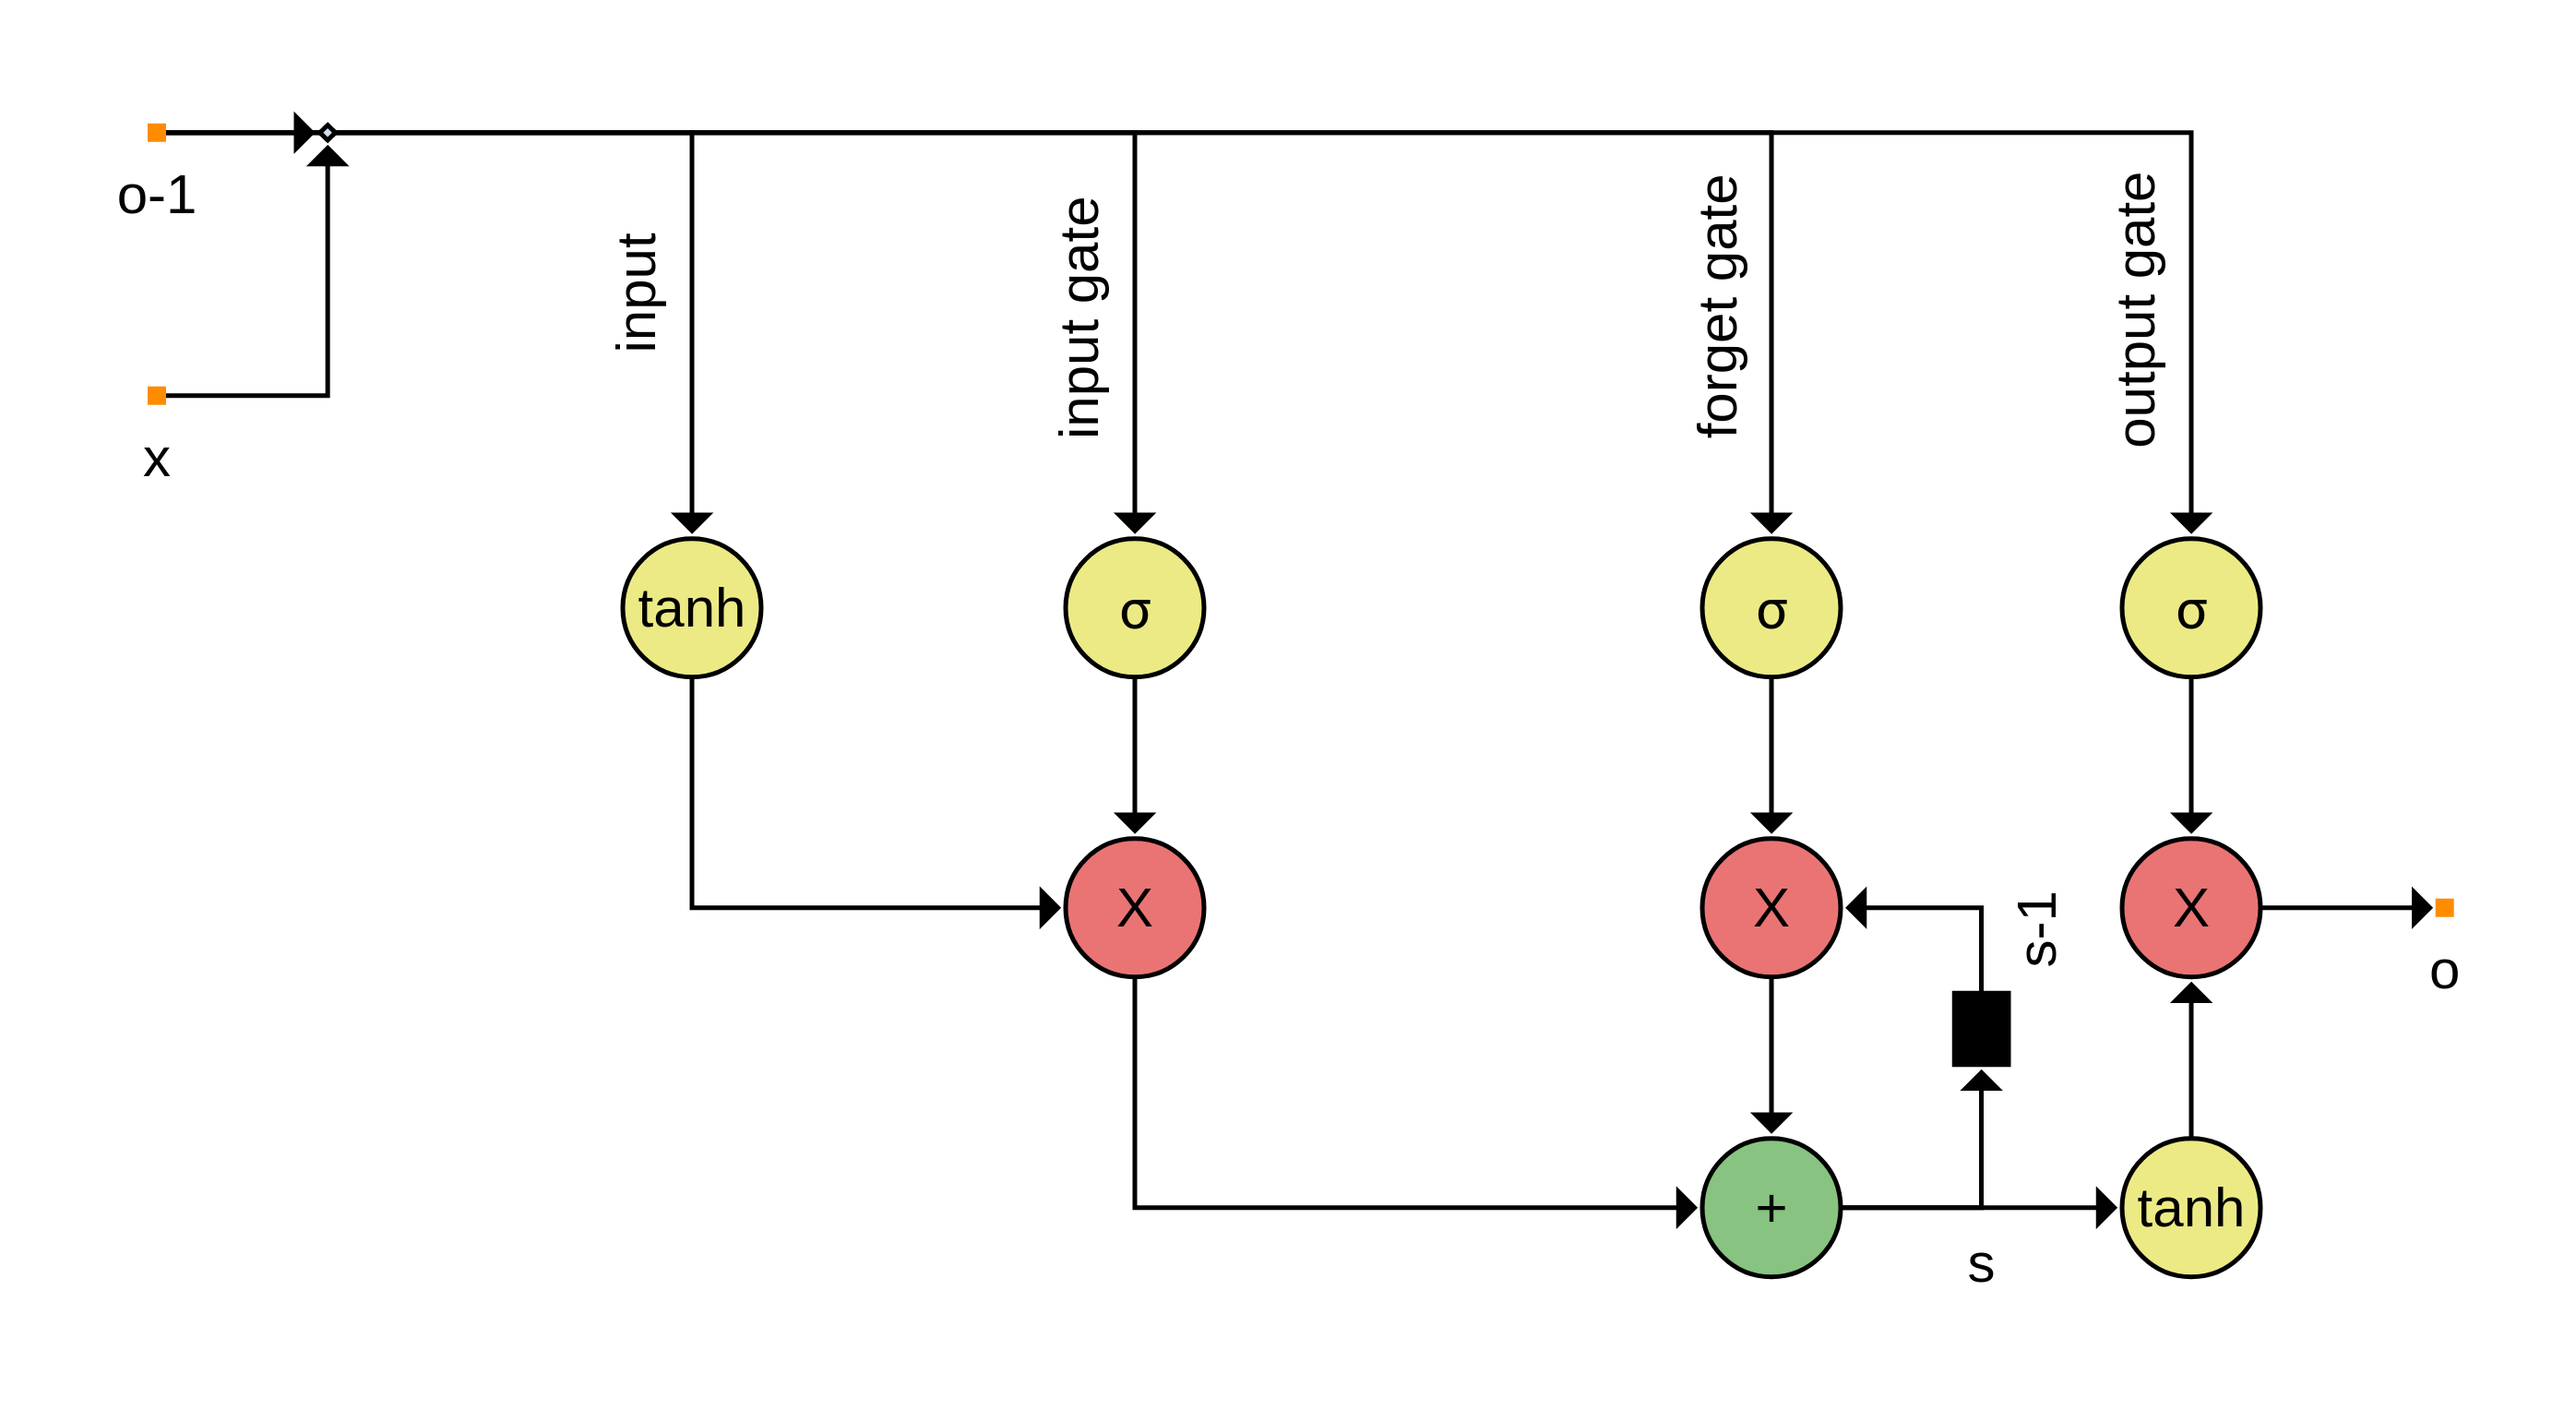
\includegraphics[width=\linewidth]{img/lstm.png}
	\end{figure}
\end{frame}

\section{Implementation Details}

\begin{frame}[fragile]{Dataset}
	
	\begin{block}{Conference on Computational NL Learning}
		CoNLL 2003 was a shared task on language independent named entity recognition.
	\end{block}

	Four types of Named Entities:
	\begin{itemize}
		\item Person
		\item Location
		\item Organization
		\item Miscellaneous
	\end{itemize}

\end{frame}

\begin{frame}[fragile]{Dataset}
	\begin{center}
		\begin{tabular}{l | l | l | l}
			Word & POS & Syntax Chunk & NE \\
			\hline
			U.N. & NNP & I-NP & I-ORG 
\\
			official & NN & I-NP & O 
\\
			Ekeus & NNP & I-NP & I-PER \\ 
			heads & VBZ & I-VP & O 
\\
			for & IN & I-PP & O \\
			Baghdad & NNP & I-NP & I-LOC \\ 
			. & . & O & O \\
		\end{tabular}
	\end{center}
\end{frame}

\begin{frame}[fragile]{Conditional Random Fields}
	Library:
	\begin{itemize}
		\item pycrfsuite
	\end{itemize}

	Features should describe characteristics of named entities.
	
	\begin{itemize}
		\item Word Features
		\item Sentence \& Collection Features
		\item Dictionary Features
		\item Features from unsupervised ML algorithms
	\end{itemize}
\end{frame}

\begin{frame}[fragile]{Word Features}
	\begin{itemize}
		\item length of word
		\item the word starts with an upper-case letter
		\item the word contains an upper-case letter
		\item the word contains a digit
		\item the word contains a special character (-, /, etc.)
		\item word shape: 'Word' $\rightarrow$ 'Aa+', 'WORD' $\rightarrow$ 'A+', '2019-12-12' $\rightarrow$ '9999\#99\#99'
	\end{itemize}
\end{frame}

\begin{frame}[fragile]{Sentence \& Collection Features}
	\begin{itemize}
		\item position of word in sentence
		\item number of occurrences in collection
	\end{itemize}
\end{frame}

\begin{frame}[fragile]{Dictionary Features}
	The word is contained in:
	\begin{itemize}
		\item stop-words list
		\item name list
		\item word list
		\item wordnet
	\end{itemize}
\end{frame}

\begin{frame}[fragile]{Features from unsupervised ML algorithms}
	\begin{itemize}
		\item brown cluster
		\item LDA topic
		\item w2c cluster
	\end{itemize}
\end{frame}

\begin{frame}[fragile]{LSTM Network}
	\begin{figure}
		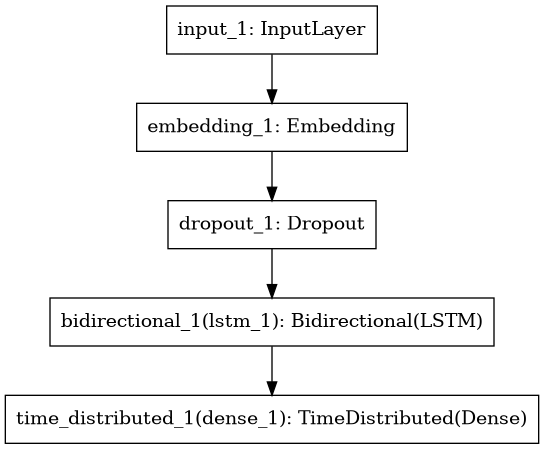
\includegraphics[width=0.8\textheight]{img/lstm_model.png}
	\end{figure}
\end{frame}

\begin{frame}[fragile]{The best of both worlds?}
	Combine the LSTM approach with CRF by adding a CRF layer at bottom.
	\begin{figure}
		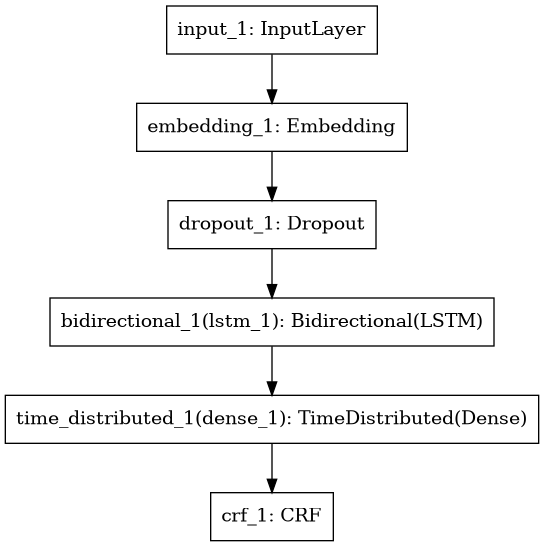
\includegraphics[width=0.65\textheight]{img/lstm_crf_model.png}
	\end{figure}
\end{frame}


\section{Evaluation and Comparison}

\section{Conclusion}


%\printbibliography

\end{document}